\documentclass{article}

% content/resources/templates/preamble.tex
\usepackage[margin=0.6in]{geometry}
\author{Milav Dabgar}
\usepackage{amsmath,amssymb,amsthm}
\usepackage{booktabs}
\usepackage{multirow}
\usepackage{xcolor}
\usepackage{tcolorbox}
\tcbuselibrary{breakable,skins}
\usepackage[colorlinks=true,linkcolor=blue]{hyperref}
\usepackage{titlesec}
\usepackage{enumitem}
\usepackage{tikz}
\usepackage{pgfplots}
\usepackage{circuitikz}
\usepackage[version=4]{mhchem}
\usepackage{longtable}
\usepackage{array}
\usepackage{float}
\usepackage{caption}
\usepackage{listings}

\lstset{
  basicstyle=\small\ttfamily,
  breaklines=true,
  breakatwhitespace=false,
  postbreak=\mbox{\textcolor{red}{$\hookrightarrow$}\space},
  float=false,
  numbers=left,
  numberstyle=\tiny\color{gray},
  numbersep=10pt,
  xleftmargin=2em,
  keywordstyle=\color{blue},
  commentstyle=\color{green!60!black},
  stringstyle=\color{purple},
  backgroundcolor=\color{gray!5},
  showstringspaces=false,
  tabsize=2,
  captionpos=b,
  keepspaces=true,
  columns=flexible
}

\pgfplotsset{compat=1.18}
\usetikzlibrary{shapes,arrows,positioning,calc,patterns,decorations.pathmorphing,decorations.markings,arrows.meta}

% Color scheme
\definecolor{headcolor}{RGB}{0,102,204}
\definecolor{keycolor}{RGB}{220,20,60}
\definecolor{solutioncolor}{RGB}{34,139,34}
\definecolor{mnemoniccolor}{RGB}{148,0,211}
\definecolor{codecolor}{RGB}{0,0,100}

% Spacing
\setlength{\parskip}{3pt}
\setlist[itemize]{nosep}
\setlist[enumerate]{nosep}

% Title formatting
\titleformat{\section}{\Large\bfseries\color{headcolor}}{\thesection}{1em}{}
\titleformat{\subsection}{\large\bfseries\color{headcolor}}{\thesubsection}{1em}{}

% Pandoc tightlist compatibility
\providecommand{\tightlist}{%
  \setlength{\itemsep}{0pt}\setlength{\parskip}{0pt}}

% Pandoc longtable compatibility
\newcounter{none}
\def\thenone{}


% content/resources/templates/english-boxes.tex

% Custom environments
\newtcolorbox{solutionbox}{
 breakable,
 enhanced,
 colback=solutioncolor!5!white,
 colframe=solutioncolor!75!black,
 fonttitle=\bfseries,
 title=Solution
}

\newtcolorbox{solutionboxnobreak}{
 colback=solutioncolor!5!white,
 colframe=solutioncolor!75!black,
 fonttitle=\bfseries,
 title=Solution
}

\newtcolorbox{keyformula}{
 breakable,
 enhanced,
 colback=keycolor!5!white,
 colframe=keycolor!75!black,
 fonttitle=\bfseries,
 title=Key Formula
}

\newtcolorbox{mnemonicboxenv}{
 breakable,
 enhanced,
 colback=mnemoniccolor!5!white,
 colframe=mnemoniccolor!75!black,
 fonttitle=\bfseries,
 title=Mnemonic
}

\newcommand{\mnemonicbox}[1]{%
  \begin{mnemonicboxenv}
    #1
  \end{mnemonicboxenv}
}


% Custom commands for GTU solutions
% This file defines semantic commands for consistent formatting

% Question command with automatic formatting
\newcommand{\question}[2]{%
  \section*{Question #1}%
  \textbf{#2}%
}

% OR question variant
\newcommand{\questionor}[2]{%
  \section*{Question #1 OR}%
  \textbf{#2}%
}

% Proper table environment with caption
\newenvironment{answertable}[1]{%
  \begin{table}[htbp]
  \centering
  \caption{#1}
}{%
  \end{table}
}

% Proper figure environment for diagrams
\newenvironment{answerdiagram}[1]{%
  \begin{figure}[htbp]
  \centering
  \caption{#1}
}{%
  \end{figure}
}

% Semantic markup for key terms
\newcommand{\keyword}[1]{\textbf{#1}}
\newcommand{\code}[1]{\texttt{#1}}
\newcommand{\classname}[1]{\texttt{#1}}
\newcommand{\methodname}[1]{\texttt{#1}}

% Proper quotation marks
\newcommand{\mnemonic}[1]{``#1''}


\title{Computer Networks \& Data Communication (4361101) - Summer 2024 Solution}
\date{May 14, 2024}

\begin{document}
\maketitle

\questionmarks{1(a)}{3}{List the different Network Topologies and discuss any one in detail.}

\begin{solutionbox}

\begin{table}[H]
\centering
\begin{tabulary}{\textwidth}{CL}
\toprule
\textbf{Topology} & \textbf{Description} \\
\midrule
\textbf{Star} & All devices connected to central hub/switch \\
\textbf{Ring} & Devices connected in circular fashion \\
\textbf{Bus} & All devices connected to single cable \\
\textbf{Mesh} & Every device connected to every other device \\
\textbf{Tree} & Hierarchical structure with root node \\
\textbf{Hybrid} & Combination of two or more topologies \\
\bottomrule
\end{tabulary}
\caption{Network Topologies}
\end{table}

\textbf{Star Topology Details:}

\begin{itemize}
    \item \textbf{Central Hub}: All nodes connect to one central device
    \item \textbf{Point-to-Point}: Each connection is dedicated between node and hub
    \item \textbf{Easy Management}: Simple to install and troubleshoot
\end{itemize}

\end{solutionbox}

\begin{mnemonicbox}
\mnemonic{STAR = Single Terminal All Reach}
\end{mnemonicbox}

\questionmarks{1(b)}{4}{Explain how point-to-point and broadcast transmission technologies are used in modern communication systems with examples of real-world applications and discuss their advantages and limitations.}

\begin{solutionbox}

\begin{table}[H]
\centering
\begin{tabulary}{\textwidth}{L L L}
\toprule
\textbf{Technology} & \textbf{Point-to-Point} & \textbf{Broadcast} \\
\midrule
\textbf{Connection} & Direct link between two devices & One-to-many communication \\
\textbf{Example} & Telephone, VPN tunnels & Radio, TV, WiFi \\
\textbf{Data Flow} & Bidirectional & Unidirectional/Multidirectional \\
\bottomrule
\end{tabulary}
\caption{Transmission Technologies Comparison}
\end{table}

\textbf{Point-to-Point Applications:}
\begin{itemize}
    \item \textbf{Dedicated Lines}: Leased lines between offices
    \item \textbf{Satellite Links}: Ground station to satellite communication
    \item \textbf{Cable Modems}: Home to ISP connection
\end{itemize}

\textbf{Broadcast Applications:}
\begin{itemize}
    \item \textbf{WiFi Networks}: Router broadcasts to multiple devices
    \item \textbf{Television}: One transmitter to many receivers
\end{itemize}

\end{solutionbox}

\begin{mnemonicbox}
\mnemonic{P2P = Private Path, Broadcast = Big Audience}
\end{mnemonicbox}

\questionmarks{1(c)}{7}{Describe OSI model with function of all layers.}

\begin{solutionbox}

\begin{table}[H]
\centering
\begin{tabulary}{\textwidth}{C L L}
\toprule
\textbf{Layer} & \textbf{Name} & \textbf{Function} \\
\midrule
\textbf{7} & Application & User interface, network services \\
\textbf{6} & Presentation & Data encryption, compression, formatting \\
\textbf{5} & Session & Establishes, manages, terminates sessions \\
\textbf{4} & Transport & Reliable data transfer, error correction \\
\textbf{3} & Network & Routing, logical addressing (IP) \\
\textbf{2} & Data Link & Frame formatting, error detection \\
\textbf{1} & Physical & Bit transmission, electrical signals \\
\bottomrule
\end{tabulary}
\caption{OSI Model Layers}
\end{table}

\begin{figure}[H]
\centering
\begin{tikzpicture}[node distance=0.8cm]
    \node (app) [gtu block, minimum width=5cm] {7. Application Layer};
    \node (pres) [gtu block, minimum width=5cm, below=of app] {6. Presentation Layer};
    \node (sess) [gtu block, minimum width=5cm, below=of pres] {5. Session Layer};
    \node (trans) [gtu block, minimum width=5cm, below=of sess] {4. Transport Layer};
    \node (net) [gtu block, minimum width=5cm, below=of trans] {3. Network Layer};
    \node (dl) [gtu block, minimum width=5cm, below=of net] {2. Data Link Layer};
    \node (phy) [gtu block, minimum width=5cm, below=of dl] {1. Physical Layer};
    
    \draw[gtu arrow] (app) -- (pres);
    \draw[gtu arrow] (pres) -- (sess);
    \draw[gtu arrow] (sess) -- (trans);
    \draw[gtu arrow] (trans) -- (net);
    \draw[gtu arrow] (net) -- (dl);
    \draw[gtu arrow] (dl) -- (phy);
    
    \node [right=of app, xshift=1cm] (upper) {Upper Layers (Software)};
    \node [right=of phy, xshift=1cm] (lower) {Lower Layers (Hardware)};
    
    \draw[dashed] (app.east) -- (upper.west);
    \draw[dashed] (phy.east) -- (lower.west);
\end{tikzpicture}
\caption{OSI Model Stack}
\end{figure}

\textbf{Key Functions:}
\begin{itemize}
    \item \textbf{Upper Layers (5-7)}: Handle application-related services
    \item \textbf{Lower Layers (1-4)}: Handle data transmission and routing
    \item \textbf{Encapsulation}: Each layer adds its own header
\end{itemize}

\end{solutionbox}

\begin{mnemonicbox}
\mnemonic{All People Seem To Need Data Processing}
\end{mnemonicbox}

\questionmarks{1(c OR)}{7}{Write a functional description of all layer of TCP/IP model.}

\begin{solutionbox}

\begin{table}[H]
\centering
\begin{tabulary}{\textwidth}{C L L L}
\toprule
\textbf{Layer} & \textbf{Name} & \textbf{Function} & \textbf{Protocols} \\
\midrule
\textbf{4} & Application & User services, applications & HTTP, FTP, SMTP, DNS \\
\textbf{3} & Transport & End-to-end communication & TCP, UDP \\
\textbf{2} & Internet & Routing, logical addressing & IP, ICMP, ARP \\
\textbf{1} & Network Access & Physical transmission & Ethernet, WiFi \\
\bottomrule
\end{tabulary}
\caption{TCP/IP Model Layers}
\end{table}

\begin{figure}[H]
\centering
\begin{tikzpicture}[node distance=1cm]
    \node (app) [gtu block, fill=purple!10, minimum width=6cm] {Application Layer};
    \node (trans) [gtu block, fill=blue!10, minimum width=6cm, below=of app] {Transport Layer};
    \node (net) [gtu block, fill=green!10, minimum width=6cm, below=of trans] {Internet Layer};
    \node (link) [gtu block, fill=orange!10, minimum width=6cm, below=of net] {Network Access Layer};

    \draw[gtu arrow] (app) -- (trans);
    \draw[gtu arrow] (trans) -- (net);
    \draw[gtu arrow] (net) -- (link);
\end{tikzpicture}
\caption{TCP/IP Model Stack}
\end{figure}

\textbf{Layer Functions:}
\begin{itemize}
    \item \textbf{Application}: Provides network services to applications
    \item \textbf{Transport}: Ensures reliable or unreliable delivery
    \item \textbf{Internet}: Routes packets across networks using IP addresses
    \item \textbf{Network Access}: Handles physical transmission media
\end{itemize}

\end{solutionbox}

\begin{mnemonicbox}
\mnemonic{Applications Transport Internet Networks}
\end{mnemonicbox}


\questionmarks{2(a)}{3}{Describe Function of firewall in network security.}

\begin{solutionbox}

\textbf{Firewall Functions:}
\begin{itemize}
    \item \textbf{Packet Filtering}: Controls incoming and outgoing network traffic
    \item \textbf{Access Control}: Blocks unauthorized access attempts
    \item \textbf{Traffic Monitoring}: Logs and analyzes network activity
\end{itemize}

\textbf{Types:}
\begin{itemize}
    \item \textbf{Hardware Firewall}: Physical device protecting entire network
    \item \textbf{Software Firewall}: Program installed on individual computers
    \item \textbf{Stateful Inspection}: Tracks connection states and contexts
\end{itemize}

\end{solutionbox}

\begin{mnemonicbox}
\mnemonic{Firewall = Filter, Access, Monitor}
\end{mnemonicbox}

\questionmarks{2(b)}{4}{Compare FDDI (Fiber Distributed Data Interface) and CDDI (Copper Distributed Data Interface) in terms of their key characteristics, advantages, and applications.}

\begin{solutionbox}

\begin{table}[H]
\centering
\begin{tabulary}{\textwidth}{L L L}
\toprule
\textbf{Feature} & \textbf{FDDI} & \textbf{CDDI} \\
\midrule
\textbf{Medium} & Optical fiber & Twisted pair copper \\
\textbf{Speed} & 100 Mbps & 100 Mbps \\
\textbf{Distance} & Up to 200 km & Up to 100 meters \\
\textbf{Cost} & Higher & Lower \\
\textbf{Security} & Higher (difficult to tap) & Lower (easier to tap) \\
\textbf{Installation} & Complex & Simple \\
\bottomrule
\end{tabulary}
\caption{FDDI vs CDDI Comparison}
\end{table}

\textbf{FDDI Advantages:}
\begin{itemize}
    \item \textbf{Long Distance}: Supports campus-wide networks
    \item \textbf{High Security}: Immune to electromagnetic interference
    \item \textbf{Reliability}: Better error detection and recovery
\end{itemize}

\textbf{CDDI Advantages:}
\begin{itemize}
    \item \textbf{Cost Effective}: Uses existing copper infrastructure
    \item \textbf{Easy Installation}: Standard twisted pair cabling
    \item \textbf{Compatibility}: Works with existing network equipment
\end{itemize}

\end{solutionbox}

\begin{mnemonicbox}
\mnemonic{FDDI = Fiber Distance, CDDI = Copper Cost}
\end{mnemonicbox}

\questionmarks{2(c)}{7}{Explain and distinguish Ethernet, Fast Ethernet, Gigabit Ethernet.}

\begin{solutionbox}

\begin{table}[H]
\centering
\begin{tabulary}{\textwidth}{L L L L L}
\toprule
\textbf{Type} & \textbf{Speed} & \textbf{Standard} & \textbf{Cable Type} & \textbf{Distance} \\
\midrule
\textbf{Ethernet} & 10 Mbps & 802.3 & Coax/UTP & 100m \\
\textbf{Fast Ethernet} & 100 Mbps & 802.3u & UTP Cat5 & 100m \\
\textbf{Gigabit Ethernet} & 1000 Mbps & 802.3z/ab & Cat5e/6, Fiber & 100m/5km \\
\bottomrule
\end{tabulary}
\caption{Ethernet Evolution Comparison}
\end{table}

\begin{figure}[H]
\centering
\begin{tikzpicture}[node distance=1.5cm]
    \node (eth) [gtu block] {Ethernet\\10 Mbps};
    \node (fast) [gtu block, right=of eth] {Fast Ethernet\\100 Mbps};
    \node (gig) [gtu block, right=of fast] {Gigabit Ethernet\\1000 Mbps};

    \draw[gtu arrow] (eth) -- (fast);
    \draw[gtu arrow] (fast) -- (gig);
\end{tikzpicture}
\caption{Evolution of Ethernet Standards}
\end{figure}

\textbf{Key Differences:}
\begin{itemize}
    \item \textbf{Speed Evolution}: 10x increase at each generation
    \item \textbf{Media Support}: From coax to twisted pair to fiber
    \item \textbf{Applications}: LAN backbone, server connections, desktop
    \item \textbf{Backward Compatibility}: Newer standards support older devices
\end{itemize}

\textbf{Standards:}
\begin{itemize}
    \item \textbf{10Base-T}: 10 Mbps over twisted pair
    \item \textbf{100Base-TX}: 100 Mbps over Category 5 UTP
    \item \textbf{1000Base-T}: 1 Gbps over Category 5e/6 UTP
\end{itemize}

\end{solutionbox}

\begin{mnemonicbox}
\mnemonic{Every Fast Gigabit = 10, 100, 1000}
\end{mnemonicbox}

\questionmarks{2(a OR)}{3}{Explain its role and function of router within a network infrastructure.}

\begin{solutionbox}

\textbf{Router Functions:}
\begin{itemize}
    \item \textbf{Packet Forwarding}: Routes data packets between different networks
    \item \textbf{Path Determination}: Selects best route using routing tables
    \item \textbf{Network Isolation}: Separates broadcast domains
\end{itemize}

\textbf{Key Roles:}
\begin{itemize}
    \item \textbf{Inter-network Communication}: Connects LANs to WANs
    \item \textbf{Traffic Management}: Controls data flow between networks
    \item \textbf{Protocol Translation}: Converts between different network protocols
\end{itemize}

\end{solutionbox}

\begin{mnemonicbox}
\mnemonic{Router = Route, Isolate, Connect}
\end{mnemonicbox}

\questionmarks{2(b OR)}{4}{Explain the structure of FDDI (Fiber Distributed Data Interface) and give its advantages.}

\begin{solutionbox}

\textbf{FDDI Structure:}

\begin{figure}[H]
\centering
\begin{tikzpicture}[node distance=2.5cm, auto]
    % Nodes
    \node (A) [gtu state] {Node\\A};
    \node (B) [gtu state, right=of A] {Node\\B};
    \node (C) [gtu state, below=of B] {Node\\C};
    \node (D) [gtu state, left=of C] {Node\\D};

    % Primary Ring (Clockwise) - Outer
    \draw[gtu arrow, thick, blue] (A.north east) to[bend left=20] (B.north west);
    \draw[gtu arrow, thick, blue] (B.south east) to[bend left=20] (C.north east);
    \draw[gtu arrow, thick, blue] (C.south west) to[bend left=20] (D.south east);
    \draw[gtu arrow, thick, blue] (D.north west) to[bend left=20] (A.south west);

    % Secondary Ring (Counter-Clockwise) - Inner
    \draw[gtu arrow, dashed, red] (B.south west) to[bend left=20] (A.south east);
    \draw[gtu arrow, dashed, red] (A.south east) to[bend left=20] (D.north east);
    \draw[gtu arrow, dashed, red] (D.north east) to[bend left=20] (C.south west);
    \draw[gtu arrow, dashed, red] (C.north west) to[bend left=20] (B.south west);
    
    % Legend
    \node[right=of B, align=left, xshift=1cm] {
        \textcolor{blue}{\textbf{---}} Primary Ring (Data) \\
        \textcolor{red}{\textbf{- -}} Secondary Ring (Backup)
    };
\end{tikzpicture}
\caption{FDDI Dual Ring Structure}
\end{figure}
\textbf{Note}: The above diagram is a simplified representation. In reality, FDDI uses two counter-rotating rings.

\textbf{Components:}
\begin{itemize}
    \item \textbf{Dual Ring}: Primary and secondary rings for redundancy
    \item \textbf{Token Passing}: Uses token for media access control
    \item \textbf{Concentrators}: Connect multiple stations to ring
\end{itemize}

\textbf{Advantages:}
\begin{itemize}
    \item \textbf{High Reliability}: Dual ring provides fault tolerance
    \item \textbf{Fast Speed}: 100 Mbps data transmission rate
    \item \textbf{Long Distance}: Supports up to 200 km ring circumference
    \item \textbf{Self-Healing}: Automatic reconfiguration when link fails
\end{itemize}

\end{solutionbox}

\begin{mnemonicbox}
\mnemonic{FDDI = Fast, Dual, Distance, Immune}
\end{mnemonicbox}

\questionmarks{2(c OR)}{7}{Explain roll of network Devices. Describe in brief about all the devices.}

\begin{solutionbox}

\begin{table}[H]
\centering
\begin{tabulary}{\textwidth}{L L L}
\toprule
\textbf{Device} & \textbf{Layer} & \textbf{Function} \\
\midrule
\textbf{Repeater} & Physical & Regenerates signals, extends distance \\
\textbf{Hub} & Physical & Connects multiple devices, shared bandwidth \\
\textbf{Bridge} & Data Link & Connects LANs, reduces collisions \\
\textbf{Switch} & Data Link & Intelligent hub, dedicated bandwidth \\
\textbf{Router} & Network & Connects different networks, routing \\
\textbf{Gateway} & All Layers & Protocol conversion, network interconnection \\
\bottomrule
\end{tabulary}
\caption{Network Devices Summary}
\end{table}

\begin{figure}[H]
\centering
\begin{tikzpicture}[node distance=1.5cm]
    \node (phy) [gtu block, fill=orange!10] {Physical Layer};
    \node (rep) [gtu block, below left=of phy, minimum width=3cm] {Repeater};
    \node (hub) [gtu block, below right=of phy, minimum width=3cm] {Hub};
    
    \node (dl) [gtu block, fill=green!10, right=of phy, xshift=2cm] {Data Link Layer};
    \node (bri) [gtu block, below left=of dl, minimum width=3cm] {Bridge};
    \node (swi) [gtu block, below right=of dl, minimum width=3cm] {Switch};
    
    \node (net) [gtu block, fill=blue!10, right=of dl, xshift=2cm] {Network Layer};
    \node (rou) [gtu block, below=of net, minimum width=3cm] {Router};

    \draw[gtu arrow] (phy) -- (rep);
    \draw[gtu arrow] (phy) -- (hub);
    \draw[gtu arrow] (dl) -- (bri);
    \draw[gtu arrow] (dl) -- (swi);
    \draw[gtu arrow] (net) -- (rou);
\end{tikzpicture}
\caption{Network Devices by Layer}
\end{figure}

\textbf{Device Functions:}
\begin{itemize}
    \item \textbf{Repeater}: Amplifies and regenerates signals
    \item \textbf{Hub}: Simple connection point for multiple devices
    \item \textbf{Bridge}: Intelligent forwarding based on MAC addresses
    \item \textbf{Switch}: High-performance bridge with multiple ports
    \item \textbf{Router}: Intelligent path selection between networks
    \item \textbf{Gateway}: Complete protocol stack conversion
\end{itemize}

\end{solutionbox}

\begin{mnemonicbox}
\mnemonic{Repeat, Hub, Bridge, Switch, Route, Gateway}
\end{mnemonicbox}


\questionmarks{3(a)}{3}{Name any three data link layer protocol and explain any one in detail.}

\begin{solutionbox}

\textbf{Data Link Layer Protocols:}
\begin{itemize}
    \item \textbf{HDLC} (High-Level Data Link Control)
    \item \textbf{PPP} (Point-to-Point Protocol)
    \item \textbf{Ethernet} (IEEE 802.3)
\end{itemize}

\textbf{HDLC Protocol Details:}
\begin{itemize}
    \item \textbf{Frame Structure}: Flag, Address, Control, Data, FCS, Flag
    \item \textbf{Error Detection}: Frame Check Sequence (FCS)
    \item \textbf{Flow Control}: Sliding window mechanism
\end{itemize}

\textbf{HDLC Frame Format:}

\begin{figure}[H]
\centering
\begin{tikzpicture}
    \node (flag1) [gtu block, minimum width=1.5cm] {Flag\\8-bit};
    \node (addr) [gtu block, right=0cm of flag1, minimum width=1.5cm] {Address\\8-bit};
    \node (ctrl) [gtu block, right=0cm of addr, minimum width=1.5cm] {Control\\8-bit};
    \node (data) [gtu block, right=0cm of ctrl, minimum width=3cm, fill=white] {Data\\Variable};
    \node (fcs) [gtu block, right=0cm of data, minimum width=1.5cm] {FCS\\16-bit};
    \node (flag2) [gtu block, right=0cm of fcs, minimum width=1.5cm] {Flag\\8-bit};
\end{tikzpicture}
\caption{HDLC Frame Structure}
\end{figure}

\end{solutionbox}

\begin{mnemonicbox}
\mnemonic{HDLC = High Data Link Control}
\end{mnemonicbox}

\questionmarks{3(b)}{4}{Explain error control and flow control at data link layer}

\begin{solutionbox}

\begin{table}[H]
\centering
\begin{tabulary}{\textwidth}{L L L}
\toprule
\textbf{Control Type} & \textbf{Purpose} & \textbf{Methods} \\
\midrule
\textbf{Error Control} & Detect and correct transmission errors & CRC, Checksum, Parity \\
\textbf{Flow Control} & Manage data transmission rate & Stop-and-Wait, Sliding Window \\
\bottomrule
\end{tabulary}
\caption{Error vs Flow Control}
\end{table}

\textbf{Error Control Methods:}
\begin{itemize}
    \item \textbf{Detection}: CRC, Checksum identify errors
    \item \textbf{Correction}: ARQ (Automatic Repeat Request)
    \item \textbf{Prevention}: Forward Error Correction (FEC)
\end{itemize}

\textbf{Flow Control Methods:}
\begin{itemize}
    \item \textbf{Stop-and-Wait}: Send one frame, wait for ACK
    \item \textbf{Sliding Window}: Send multiple frames before ACK
    \item \textbf{Buffer Management}: Prevent receiver overflow
\end{itemize}

\end{solutionbox}

\begin{mnemonicbox}
\mnemonic{Error = Detect, Flow = Control}
\end{mnemonicbox}

\questionmarks{3(c)}{7}{Compare IPv6 and IPv4.}

\begin{solutionbox}

\begin{table}[H]
\centering
\begin{tabulary}{\textwidth}{L L L}
\toprule
\textbf{Feature} & \textbf{IPv4} & \textbf{IPv6} \\
\midrule
\textbf{Address Length} & 32 bits & 128 bits \\
\textbf{Address Space} & 4.3 billion & 340 undecillion \\
\textbf{Header Size} & 20-60 bytes (variable) & 40 bytes (fixed) \\
\textbf{Notation} & Decimal (192.168.1.1) & Hex (2001:db8::1) \\
\textbf{Fragmentation} & Router and host & Host only \\
\textbf{Security} & Optional (IPSec) & Built-in (IPSec) \\
\textbf{Configuration} & Manual/DHCP & Auto-configuration \\
\bottomrule
\end{tabulary}
\caption{IPv4 vs IPv6 Comparison}
\end{table}

\textbf{IPv4 Example:} 192.168.1.100 \\
\textbf{IPv6 Example:} 2001:0db8:85a3:0000:0000:8a2e:0370:7334

\textbf{Key Differences:}
\begin{itemize}
    \item \textbf{Address Exhaustion}: IPv4 addresses nearly exhausted
    \item \textbf{Header Efficiency}: IPv6 simplified header structure
    \item \textbf{Security}: IPv6 has built-in security features
    \item \textbf{Quality of Service}: Better QoS support in IPv6
\end{itemize}

\end{solutionbox}

\begin{mnemonicbox}
\mnemonic{IPv6 = Infinite, Integrated, Improved}
\end{mnemonicbox}

\questionmarks{3(a OR)}{3}{Explain the differences between guided and unguided transmission media used in computer networks}

\begin{solutionbox}

\begin{table}[H]
\centering
\begin{tabulary}{\textwidth}{L L L}
\toprule
\textbf{Media Type} & \textbf{Guided} & \textbf{Unguided} \\
\midrule
\textbf{Definition} & Physical path exists & No physical path \\
\textbf{Examples} & Twisted pair, Coax, Fiber & Radio, Microwave, Satellite \\
\textbf{Direction} & Point-to-point & Broadcast \\
\bottomrule
\end{tabulary}
\caption{Guided vs Unguided Media}
\end{table}

\textbf{Guided Media:}
\begin{itemize}
    \item \textbf{Twisted Pair}: Telephone lines, LANs
    \item \textbf{Coaxial Cable}: Cable TV, older networks
    \item \textbf{Fiber Optic}: High-speed, long-distance
\end{itemize}

\textbf{Unguided Media:}
\begin{itemize}
    \item \textbf{Radio Waves}: WiFi, Bluetooth
    \item \textbf{Microwaves}: Point-to-point links
    \item \textbf{Infrared}: Short-range communication
\end{itemize}

\end{solutionbox}

\begin{mnemonicbox}
\mnemonic{Guided = Ground, Unguided = Air}
\end{mnemonicbox}

\questionmarks{3(b OR)}{4}{Describe circuit switching and packet switching.}

\begin{solutionbox}

\begin{table}[H]
\centering
\begin{tabulary}{\textwidth}{L L L}
\toprule
\textbf{Feature} & \textbf{Circuit Switching} & \textbf{Packet Switching} \\
\midrule
\textbf{Connection} & Dedicated path established & No dedicated path \\
\textbf{Resource Allocation} & Fixed bandwidth & Shared resources \\
\textbf{Example} & Traditional telephone & Internet \\
\textbf{Delay} & Constant & Variable \\
\bottomrule
\end{tabulary}
\caption{Circuit vs Packet Switching}
\end{table}

\textbf{Circuit Switching:}
\begin{itemize}
    \item \textbf{Setup Phase}: Establishes dedicated connection
    \item \textbf{Data Transfer}: Continuous transmission
    \item \textbf{Teardown}: Releases connection resources
\end{itemize}

\textbf{Packet Switching:}
\begin{itemize}
    \item \textbf{Store-and-Forward}: Packets stored at intermediate nodes
    \item \textbf{Dynamic Routing}: Each packet routed independently
    \item \textbf{Resource Sharing}: Bandwidth shared among users
\end{itemize}

\end{solutionbox}

\begin{mnemonicbox}
\mnemonic{Circuit = Continuous, Packet = Pieces}
\end{mnemonicbox}

\questionmarks{3(c OR)}{7}{Explain IPv4 OR IPv6 in detail.}

\begin{solutionbox}

\textbf{IPv4 Address Structure:}
\begin{itemize}
    \item \textbf{32-bit Address}: Divided into 4 octets
    \item \textbf{Dotted Decimal}: 192.168.1.1 format
    \item \textbf{Network + Host}: Address split into network and host portions
\end{itemize}

\begin{table}[H]
\centering
\begin{tabulary}{\textwidth}{C C C C L}
\toprule
\textbf{Class} & \textbf{Range} & \textbf{Network Bits} & \textbf{Host Bits} & \textbf{Use} \\
\midrule
\textbf{A} & 1-126 & 8 & 24 & Large networks \\
\textbf{B} & 128-191 & 16 & 16 & Medium networks \\
\textbf{C} & 192-223 & 24 & 8 & Small networks \\
\bottomrule
\end{tabulary}
\caption{IPv4 Classes}
\end{table}

\textbf{Special Addresses:}
\begin{itemize}
    \item \textbf{Loopback}: 127.0.0.1 (local host)
    \item \textbf{Private}: 192.168.x.x, 10.x.x.x, 172.16-31.x.x
    \item \textbf{Broadcast}: 255.255.255.255
\end{itemize}

\textbf{IPv4 Header:}

\begin{figure}[H]
\centering
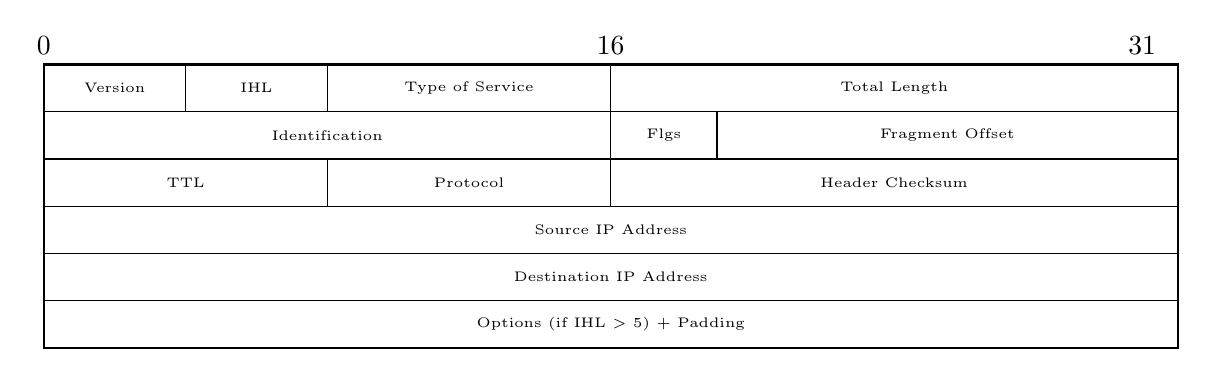
\begin{tikzpicture}[x=0.45cm, y=0.6cm]
    \draw[thick] (0,0) rectangle (32, -6);
    
    % Horizontal lines
    \foreach \y in {-1,-2,-3,-4,-5}
        \draw (0,\y) -- (32,\y);
        
    % Vertical lines for row 1
    \draw (4,0) -- (4,-1);
    \draw (8,0) -- (8,-1);
    \draw (16,0) -- (16,-1);
    
    % Vertical lines for row 2
    \draw (16,-1) -- (16,-2);
    \draw (19,-1) -- (19,-2);
    
    % Vertical lines for row 3
    \draw (8,-2) -- (8,-3);
    \draw (16,-2) -- (16,-3);
    
    % Labels Row 1
    \node at (2,-0.5) {\tiny Version};
    \node at (6,-0.5) {\tiny IHL};
    \node at (12,-0.5) {\tiny Type of Service};
    \node at (24,-0.5) {\tiny Total Length};
    
    % Labels Row 2
    \node at (8,-1.5) {\tiny Identification};
    \node at (17.5,-1.5) {\tiny Flgs};
    \node at (25.5,-1.5) {\tiny Fragment Offset};
    
    % Labels Row 3
    \node at (4,-2.5) {\tiny TTL};
    \node at (12,-2.5) {\tiny Protocol};
    \node at (24,-2.5) {\tiny Header Checksum};
    
    % Labels Row 4 & 5
    \node at (16,-3.5) {\tiny Source IP Address};
    \node at (16,-4.5) {\tiny Destination IP Address};
    
    % Row 6
    \node at (16,-5.5) {\tiny Options (if IHL > 5) + Padding};
    
    % Scales
    \node[above] at (0,0) {0};
    \node[above] at (16,0) {16};
    \node[above] at (31,0) {31};
\end{tikzpicture}
\caption{IPv4 Header Structure}
\end{figure}

\end{solutionbox}

\begin{mnemonicbox}
\mnemonic{IPv4 = 4 octets, 32 bits, Classes A-C}
\end{mnemonicbox}


\questionmarks{4(a)}{3}{Give full name of ARP and RARP and describe them.}

\begin{solutionbox}

\textbf{Full Names:}
\begin{itemize}
    \item \textbf{ARP}: Address Resolution Protocol
    \item \textbf{RARP}: Reverse Address Resolution Protocol
\end{itemize}

\begin{table}[H]
\centering
\begin{tabulary}{\textwidth}{L L}
\toprule
\textbf{Protocol} & \textbf{Function} \\
\midrule
\textbf{ARP} & Maps IP address to MAC address \\
\textbf{RARP} & Maps MAC address to IP address \\
\bottomrule
\end{tabulary}
\caption{ARP vs RARP}
\end{table}

\textbf{ARP Process:}
\begin{itemize}
    \item \textbf{Request}: "Who has IP 192.168.1.1?"
    \item \textbf{Reply}: "192.168.1.1 is at MAC 00:1A:2B:3C:4D:5E"
    \item \textbf{Cache}: Stores mappings for future use
\end{itemize}

\textbf{RARP Process:}
\begin{itemize}
    \item \textbf{Diskless Workstations}: Get IP from server
    \item \textbf{Broadcast Request}: Sends MAC address
    \item \textbf{Server Response}: Returns assigned IP address
\end{itemize}

\end{solutionbox}

\begin{mnemonicbox}
\mnemonic{ARP = Address to MAC, RARP = Reverse}
\end{mnemonicbox}

\questionmarks{4(b)}{4}{Describe DSL technology with its advantages and limitations.}

\begin{solutionbox}

\textbf{DSL (Digital Subscriber Line):}

\begin{table}[H]
\centering
\begin{tabulary}{\textwidth}{L L L}
\toprule
\textbf{Type} & \textbf{Speed} & \textbf{Distance} \\
\midrule
\textbf{ADSL} & Up to 8 Mbps & 5.5 km \\
\textbf{VDSL} & Up to 52 Mbps & 1.5 km \\
\textbf{SDSL} & Up to 2 Mbps & 3 km \\
\bottomrule
\end{tabulary}
\caption{DSL Types}
\end{table}

\textbf{Advantages:}
\begin{itemize}
    \item \textbf{Existing Infrastructure}: Uses telephone lines
    \item \textbf{Always-On}: Continuous internet connection
    \item \textbf{Voice + Data}: Simultaneous phone and internet
    \item \textbf{Cost-Effective}: Affordable for home users
\end{itemize}

\textbf{Limitations:}
\begin{itemize}
    \item \textbf{Distance Dependent}: Speed decreases with distance
    \item \textbf{Upload Speed}: Lower than download speed (ADSL)
    \item \textbf{Line Quality}: Affected by copper wire condition
    \item \textbf{Availability}: Not available in all areas
\end{itemize}

\end{solutionbox}

\begin{mnemonicbox}
\mnemonic{DSL = Digital Subscriber Line}
\end{mnemonicbox}

\questionmarks{4(c)}{7}{Role of DNS- Domain Name System.}

\begin{solutionbox}

\textbf{DNS Functions:}
\begin{itemize}
    \item \textbf{Name Resolution}: Converts domain names to IP addresses
    \item \textbf{Hierarchical Structure}: Organized in tree-like structure
    \item \textbf{Distributed Database}: Information stored across multiple servers
\end{itemize}

\begin{figure}[H]
\centering
\begin{tikzpicture}[level distance=1.5cm,
  level 1/.style={sibling distance=5cm},
  level 2/.style={sibling distance=2.5cm},
  level 3/.style={sibling distance=2.5cm}]
  \node [gtu root] {Root (.)}
    child {node [gtu child] {.com}
      child {node [gtu child] {google.com}
        child {node [gtu child] {mail} edge from parent node[left, font=\tiny] {sub}}
        child {node [gtu child] {drive} edge from parent node[right, font=\tiny] {sub}}
      }
      child {node [gtu child] {yahoo.com}}
    }
    child {node [gtu child] {.org}};
\end{tikzpicture}
\caption{DNS Hierarchical Structure}
\end{figure}

\textbf{DNS Hierarchy:}
\begin{itemize}
    \item \textbf{Root Domain}: Highest level (.)
    \item \textbf{Top-Level Domain}: .com, .org, .net, .edu
    \item \textbf{Second-Level Domain}: google.com, yahoo.com
    \item \textbf{Subdomain}: www.google.com, mail.google.com
\end{itemize}

\textbf{DNS Resolution Process:}
\begin{enumerate}
    \item \textbf{Client Query}: User types www.example.com
    \item \textbf{Local DNS}: Checks local cache
    \item \textbf{Root Server}: Queries root DNS server
    \item \textbf{TLD Server}: Queries .com server
    \item \textbf{Authoritative Server}: Gets IP address
    \item \textbf{Response}: Returns IP to client
\end{enumerate}

\textbf{DNS Record Types:}
\begin{itemize}
    \item \textbf{A Record}: Maps domain to IPv4 address
    \item \textbf{AAAA Record}: Maps domain to IPv6 address
    \item \textbf{CNAME}: Canonical name (alias)
    \item \textbf{MX}: Mail exchange server
    \item \textbf{NS}: Name server records
\end{itemize}

\end{solutionbox}

\begin{mnemonicbox}
\mnemonic{DNS = Domain Name System}
\end{mnemonicbox}

\questionmarks{4(a OR)}{3}{Give full name of DHCP and BOOTP. and describe them.}

\begin{solutionbox}

\textbf{Full Names:}
\begin{itemize}
    \item \textbf{DHCP}: Dynamic Host Configuration Protocol
    \item \textbf{BOOTP}: Bootstrap Protocol
\end{itemize}

\begin{table}[H]
\centering
\begin{tabulary}{\textwidth}{L L}
\toprule
\textbf{Protocol} & \textbf{Function} \\
\midrule
\textbf{DHCP} & Automatically assigns IP addresses \\
\textbf{BOOTP} & Provides IP address to diskless workstations \\
\bottomrule
\end{tabulary}
\caption{DHCP vs BOOTP}
\end{table}

\textbf{DHCP Process:}
\begin{itemize}
    \item \textbf{Discover}: Client broadcasts request
    \item \textbf{Offer}: Server offers IP address
    \item \textbf{Request}: Client requests specific IP
    \item \textbf{Acknowledge}: Server confirms assignment
\end{itemize}

\textbf{BOOTP Process:}
\begin{itemize}
    \item \textbf{Static Configuration}: Pre-configured IP assignments
    \item \textbf{Diskless Boot}: Workstations boot from network
    \item \textbf{Server Response}: Provides IP and boot information
\end{itemize}

\end{solutionbox}

\begin{mnemonicbox}
\mnemonic{DHCP = Dynamic, BOOTP = Bootstrap}
\end{mnemonicbox}

\questionmarks{4(b OR)}{4}{Differences Between Virtual Circuits and Datagram Networks.}

\begin{solutionbox}

\begin{table}[H]
\centering
\begin{tabulary}{\textwidth}{L L L}
\toprule
\textbf{Feature} & \textbf{Virtual Circuits} & \textbf{Datagram Networks} \\
\midrule
\textbf{Connection} & Connection-oriented & Connectionless \\
\textbf{Setup} & Requires setup phase & No setup required \\
\textbf{Routing} & Same path for all packets & Independent routing \\
\textbf{Order} & Packets arrive in order & May arrive out of order \\
\textbf{Reliability} & More reliable & Less reliable \\
\textbf{Overhead} & Higher setup overhead & Lower per-packet overhead \\
\bottomrule
\end{tabulary}
\caption{Virtual Circuits vs Datagram Networks}
\end{table}

\textbf{Virtual Circuits:}
\begin{itemize}
    \item \textbf{Path Establishment}: Creates virtual connection
    \item \textbf{State Information}: Maintains connection state
    \item \textbf{Examples}: ATM, Frame Relay
\end{itemize}

\textbf{Datagram Networks:}
\begin{itemize}
    \item \textbf{Independent Packets}: Each packet routed separately
    \item \textbf{Stateless}: No connection state maintained
    \item \textbf{Examples}: Internet Protocol (IP)
\end{itemize}

\end{solutionbox}

\begin{mnemonicbox}
\mnemonic{Virtual = Connection, Datagram = Independent}
\end{mnemonicbox}

\questionmarks{4(c OR)}{7}{Explain TCP and UDP protocol in transport layer}

\begin{solutionbox}

\begin{table}[H]
\centering
\begin{tabulary}{\textwidth}{L L L}
\toprule
\textbf{Feature} & \textbf{TCP} & \textbf{UDP} \\
\midrule
\textbf{Connection} & Connection-oriented & Connectionless \\
\textbf{Reliability} & Reliable & Unreliable \\
\textbf{Header Size} & 20 bytes & 8 bytes \\
\textbf{Flow Control} & Yes & No \\
\textbf{Error Control} & Yes & Basic \\
\textbf{Speed} & Slower & Faster \\
\bottomrule
\end{tabulary}
\caption{TCP vs UDP}
\end{table}

\textbf{TCP (Transmission Control Protocol):}
\begin{itemize}
    \item \textbf{Three-Way Handshake}: SYN, SYN-ACK, ACK
    \item \textbf{Flow Control}: Sliding window mechanism
    \item \textbf{Error Recovery}: Retransmission of lost packets
    \item \textbf{Congestion Control}: Prevents network overload
\end{itemize}

\textbf{TCP Header:}
\begin{figure}[H]
\centering
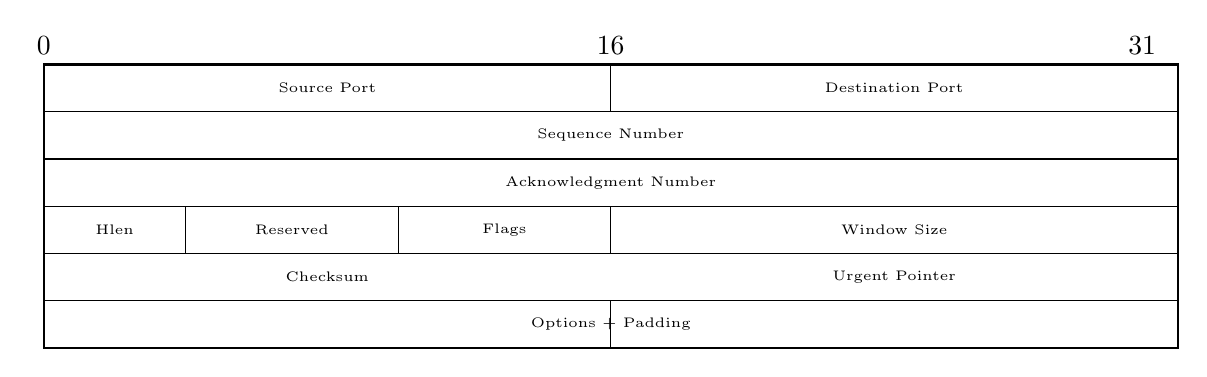
\begin{tikzpicture}[x=0.45cm, y=0.6cm]
  \draw[thick] (0,0) rectangle (32, -6);
  
  \foreach \y in {-1,-2,-3,-4,-5} \draw (0,\y) -- (32,\y);
  \draw (16,0) -- (16,-1);
  \draw (32,0) -- (32,-1);

  \draw (4,-3) -- (4,-4);
  \draw (10,-3) -- (10,-4);
  \draw (16,-3) -- (16,-4);
  
  \draw (16,-5) -- (16,-6);
  
  \node at (8,-0.5) {\tiny Source Port};
  \node at (24,-0.5) {\tiny Destination Port};
  \node at (16,-1.5) {\tiny Sequence Number};
  \node at (16,-2.5) {\tiny Acknowledgment Number};
  
  \node at (2,-3.5) {\tiny Hlen};
  \node at (7,-3.5) {\tiny Reserved};
  \node at (13,-3.5) {\tiny Flags};
  \node at (24,-3.5) {\tiny Window Size};
  
  \node at (8,-4.5) {\tiny Checksum};
  \node at (24,-4.5) {\tiny Urgent Pointer};
  
  \node at (16,-5.5) {\tiny Options + Padding};
  
   % Scales
  \node[above] at (0,0) {0};
  \node[above] at (16,0) {16};
  \node[above] at (31,0) {31};
\end{tikzpicture}
\caption{TCP Header Structure}
\end{figure}

\textbf{UDP (User Datagram Protocol):}
\begin{itemize}
    \item \textbf{Simple Protocol}: Minimal overhead
    \item \textbf{Best Effort}: No guarantee of delivery
    \item \textbf{Applications}: DNS, DHCP, streaming media
    \item \textbf{Real-time Communication}: Voice, video applications
\end{itemize}

\textbf{UDP Header:}
\begin{figure}[H]
\centering
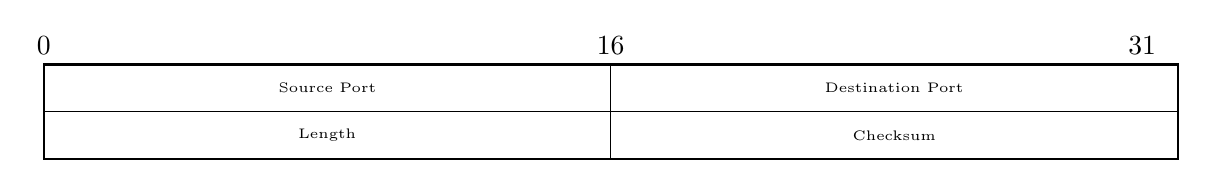
\begin{tikzpicture}[x=0.45cm, y=0.6cm]
  \draw[thick] (0,0) rectangle (32, -2);
  \foreach \y in {-1} \draw (0,\y) -- (32,\y);
  \draw (16,0) -- (16,-1);
  \draw (16,-1) -- (16,-2);
  
  \node at (8,-0.5) {\tiny Source Port};
  \node at (24,-0.5) {\tiny Destination Port};
  \node at (8,-1.5) {\tiny Length};
  \node at (24,-1.5) {\tiny Checksum};
  
  % Scales
  \node[above] at (0,0) {0};
  \node[above] at (16,0) {16};
  \node[above] at (31,0) {31};
\end{tikzpicture}
\caption{UDP Header Structure}
\end{figure}

\textbf{Applications:}
\begin{itemize}
    \item \textbf{TCP}: Web browsing, email, file transfer
    \item \textbf{UDP}: Online gaming, video streaming, DNS queries
\end{itemize}

\end{solutionbox}

\begin{mnemonicbox}
\mnemonic{TCP = Reliable, UDP = Fast}
\end{mnemonicbox}


\questionmarks{5(a)}{3}{Explain any two of following. (1) WWW (2) FTP (3) SMTP}

\begin{solutionbox}

\textbf{WWW (World Wide Web):}
\begin{itemize}
    \item \textbf{HTTP Protocol}: HyperText Transfer Protocol
    \item \textbf{Web Browser}: Client software (Chrome, Firefox)
    \item \textbf{Web Server}: Serves web pages (Apache, IIS)
\end{itemize}

\textbf{FTP (File Transfer Protocol):}
\begin{itemize}
    \item \textbf{File Transfer}: Upload and download files
    \item \textbf{Two Modes}: Active and passive mode
    \item \textbf{Authentication}: Username and password required
\end{itemize}

\begin{table}[H]
\centering
\begin{tabulary}{\textwidth}{L L L}
\toprule
\textbf{Service} & \textbf{Port} & \textbf{Function} \\
\midrule
\textbf{WWW} & 80/443 & Web page delivery \\
\textbf{FTP} & 20/21 & File transfer \\
\bottomrule
\end{tabulary}
\caption{WWW vs FTP}
\end{table}

\end{solutionbox}

\begin{mnemonicbox}
\mnemonic{WWW = Web, FTP = Files}
\end{mnemonicbox}

\questionmarks{5(b)}{4}{Difference between symmetric and asymmetric encryption algorithms.}

\begin{solutionbox}

\begin{table}[H]
\centering
\begin{tabulary}{\textwidth}{L L L}
\toprule
\textbf{Feature} & \textbf{Symmetric} & \textbf{Asymmetric} \\
\midrule
\textbf{Keys} & Same key for encryption and decryption & Different keys (public/private) \\
\textbf{Speed} & Fast & Slow \\
\textbf{Key Distribution} & Difficult & Easy \\
\textbf{Examples} & AES, DES & RSA, ECC \\
\bottomrule
\end{tabulary}
\caption{Symmetric vs Asymmetric Encryption}
\end{table}

\textbf{Symmetric Encryption:}
\begin{itemize}
    \item \textbf{Single Key}: Same key used by sender and receiver
    \item \textbf{Key Management}: Secure key distribution required
    \item \textbf{Performance}: Fast encryption/decryption
    \item \textbf{Applications}: Bulk data encryption
\end{itemize}

\textbf{Asymmetric Encryption:}
\begin{itemize}
    \item \textbf{Key Pair}: Public key for encryption, private key for decryption
    \item \textbf{Key Distribution}: Public key can be shared openly
    \item \textbf{Performance}: Slower than symmetric
    \item \textbf{Applications}: Digital signatures, key exchange
\end{itemize}

\end{solutionbox}

\begin{mnemonicbox}
\mnemonic{Symmetric = Same, Asymmetric = Different}
\end{mnemonicbox}

\questionmarks{5(c)}{7}{Define the terms ``encryption'' and ``decryption'' in the context of cryptography.}

\begin{solutionbox}

\textbf{Encryption:}
\begin{itemize}
    \item \textbf{Definition}: Process of converting plaintext into ciphertext
    \item \textbf{Purpose}: Protect data confidentiality
    \item \textbf{Input}: Plaintext + Key
    \item \textbf{Output}: Ciphertext
\end{itemize}

\textbf{Decryption:}
\begin{itemize}
    \item \textbf{Definition}: Process of converting ciphertext back to plaintext
    \item \textbf{Purpose}: Retrieve original data
    \item \textbf{Input}: Ciphertext + Key
    \item \textbf{Output}: Plaintext
\end{itemize}

\begin{figure}[H]
\centering
\begin{tikzpicture}[node distance=1.5cm, auto]
    \node (plain) [gtu input, minimum width=2.5cm] {Plaintext};
    \node (enc) [gtu process, right=of plain] {Encryption};
    \node (cipher) [gtu input, right=of enc, fill=gray!20, minimum width=2.5cm] {Ciphertext};
    \node (dec) [gtu process, right=of cipher] {Decryption};
    \node (plain2) [gtu input, right=of dec, minimum width=2.5cm] {Plaintext};
    
    \node (key1) [gtu start, above=of enc, fill=yellow!20] {Key};
    \node (key2) [gtu start, above=of dec, fill=yellow!20] {Key};

    \draw[gtu arrow] (plain) -- (enc);
    \draw[gtu arrow] (enc) -- (cipher);
    \draw[gtu arrow] (cipher) -- (dec);
    \draw[gtu arrow] (dec) -- (plain2);
    
    \draw[gtu arrow] (key1) -- (enc);
    \draw[gtu arrow] (key2) -- (dec);
\end{tikzpicture}
\caption{Cryptography Process}
\end{figure}

\textbf{Cryptographic Process:}
\begin{enumerate}
    \item \textbf{Sender}: Encrypts message using key
    \item \textbf{Transmission}: Sends ciphertext over network
    \item \textbf{Receiver}: Decrypts ciphertext using key
    \item \textbf{Recovery}: Gets original plaintext message
\end{enumerate}

\textbf{Types of Encryption:}
\begin{itemize}
    \item \textbf{Stream Cipher}: Encrypts one bit/byte at a time
    \item \textbf{Block Cipher}: Encrypts fixed-size blocks
\end{itemize}

\end{solutionbox}

\questionmarks{5(a OR)}{3}{Difference between IMAP and POP3}

\begin{solutionbox}

\begin{table}[H]
\centering
\begin{tabulary}{\textwidth}{L L L}
\toprule
\textbf{Feature} & \textbf{IMAP} & \textbf{POP3} \\
\midrule
\textbf{Storage} & Server-side & Client-side \\
\textbf{Access} & Multiple devices & Single device \\
\textbf{Offline} & Limited & Full access \\
\bottomrule
\end{tabulary}
\caption{IMAP vs POP3}
\end{table}

\textbf{IMAP (Internet Message Access Protocol):}
\begin{itemize}
    \item \textbf{Server Storage}: Messages remain on server
    \item \textbf{Multi-Device}: Access from multiple devices
    \item \textbf{Synchronization}: Changes sync across devices
\end{itemize}

\textbf{POP3 (Post Office Protocol 3):}
\begin{itemize}
    \item \textbf{Download}: Messages downloaded to client
    \item \textbf{Single Device}: Best for one device access
    \item \textbf{Storage}: Client manages message storage
\end{itemize}

\end{solutionbox}

\begin{mnemonicbox}
\mnemonic{IMAP = Internet Access, POP3 = Post Office}
\end{mnemonicbox}

\questionmarks{5(b OR)}{4}{Briefly describe the Information Technology (Amendment) Act, 2008, and its impact on cyber laws in India.}

\begin{solutionbox}

\textbf{IT Act 2008 Key Features:}
\begin{itemize}
    \item \textbf{Cyber Crimes}: Defines various cyber offenses
    \item \textbf{Data Protection}: Privacy and security requirements
    \item \textbf{Digital Signatures}: Legal recognition of e-signatures
    \item \textbf{Penalties}: Fines and imprisonment for violations
\end{itemize}

\textbf{Major Amendments:}
\begin{itemize}
    \item \textbf{Section 66A}: Criminalized offensive messages (later struck down)
    \item \textbf{Section 69}: Government power to intercept information
    \item \textbf{Section 72A}: Punishment for disclosure of personal information
    \item \textbf{Section 43A}: Compensation for data breach
\end{itemize}

\textbf{Impact on Cyber Laws:}
\begin{itemize}
    \item \textbf{Legal Framework}: Comprehensive cyber law structure
    \item \textbf{Business Compliance}: Data protection requirements
    \item \textbf{Individual Rights}: Privacy protection mechanisms
    \item \textbf{Law Enforcement}: Tools for investigating cyber crimes
\end{itemize}

\end{solutionbox}

\begin{mnemonicbox}
\mnemonic{IT Act = Internet Technology Act}
\end{mnemonicbox}

\questionmarks{5(c OR)}{7}{Difference between symmetric and asymmetric encryption algorithms.}

\begin{solutionbox}

\begin{table}[H]
\centering
\begin{tabulary}{\textwidth}{L L L}
\toprule
\textbf{Aspect} & \textbf{Symmetric Encryption} & \textbf{Asymmetric Encryption} \\
\midrule
\textbf{Key Usage} & Same key for encrypt/decrypt & Different keys (public/private) \\
\textbf{Key Management} & Difficult key distribution & Easy key distribution \\
\textbf{Performance} & Fast processing & Slow processing \\
\textbf{Key Length} & Shorter keys (128-256 bits) & Longer keys (1024-4096 bits) \\
\textbf{Scalability} & Poor ($n^2$ key pairs needed) & Good ($n$ key pairs needed) \\
\bottomrule
\end{tabulary}
\caption{Symmetric vs Asymmetric Detailed Comparison}
\end{table}

\textbf{Symmetric Encryption Details:}
\begin{itemize}
    \item \textbf{Algorithm Types}: Stream ciphers, Block ciphers
    \item \textbf{Key Distribution Problem}: Secure channel needed for key exchange
    \item \textbf{Applications}: Bulk data encryption, VPNs, file encryption
\end{itemize}

\textbf{Asymmetric Encryption Details:}
\begin{itemize}
    \item \textbf{Public Key Infrastructure}: PKI for key management
    \item \textbf{Digital Signatures}: Authentication and non-repudiation
    \item \textbf{Applications}: Email security, SSL/TLS, digital certificates
\end{itemize}

\begin{figure}[H]
\centering
\begin{tikzpicture}[node distance=1.5cm]
    \node (root) [gtu root] {Encryption Methods};
    \node (sym) [gtu child, below left=of root, xshift=-1cm] {Symmetric};
    \node (asym) [gtu child, below right=of root, xshift=1cm] {Asymmetric};
    
    \node (same) [gtu child, below=of sym] {Same Key};
    \node (fast) [gtu child, below=of same] {Fast Processing};
    
    \node (pair) [gtu child, below=of asym] {Key Pair};
    \node (slow) [gtu child, below=of pair] {Slow Processing};
    
    \draw[gtu arrow] (root) -- (sym);
    \draw[gtu arrow] (root) -- (asym);
    \draw[gtu arrow] (sym) -- (same);
    \draw[gtu arrow] (same) -- (fast);
    \draw[gtu arrow] (asym) -- (pair);
    \draw[gtu arrow] (pair) -- (slow);
\end{tikzpicture}
\caption{Encryption Methods Classification}
\end{figure}

\textbf{Real-world Applications:}
\begin{itemize}
    \item \textbf{Banking}: ATM transactions use symmetric encryption
    \item \textbf{E-commerce}: HTTPS uses hybrid encryption
    \item \textbf{Email}: PGP uses asymmetric for key exchange
    \item \textbf{Mobile}: WhatsApp uses end-to-end encryption
\end{itemize}

\end{solutionbox}

\begin{mnemonicbox}
\mnemonic{Symmetric = Same Speed, Asymmetric = Advanced Security}
\end{mnemonicbox}

\end{document}
